\chapter{Your First Programs}
\label{firstprogs}

% 
% 
% Copyright 2002 Jonathan Bartlett
% 
% Permission is granted to copy, distribute and/or modify this
% document under the terms of the GNU Free Documentation License,
% Version 1.1 or any later version published by the Free Software
% Foundation; with no Invariant Sections, with no Front-Cover Texts,
% and with no Back-Cover Texts.  A copy of the license is included in fdl.xml
% 

In this chapter you will learn the process for writing and building
Linux assembly-language programs.  In addition, you will learn the 
structure of assembly-language programs, and a few assembly-language
commands.  As you go through this chapter, you may want to refer also
to \autoref{instructionsappendix} and 
\autoref{gdbappendix}.

These programs may overwhelm you at first.  However, go through
them with diligence, read them and their explanations as many times
as necessary, and you will have a solid foundation of knowledge to
build on.  Please tinker around with the programs as much as you can.
Even if your tinkering does not work, every failure will help you learn.

\section{Entering in the Program}

Okay, this first program is simple.  In fact, it's not
going to do anything but exit!  It's short, but it shows
some basics about assembly language and Linux programming.
You need to enter the program in an editor exactly as written, 
with the filename \icodefilename{exit.s}.  The program follows.
Don't worry about not understanding it.  This section only deals with
typing it in and running it.  In \autoref{assemblyoutline} we
will describe how it works.

\begin{simpletyping}
\lstinputlisting{exit.s}
\end{simpletyping}

What you have typed in is called the \emph{source code\index{source code}}.
Source code is the human-readable form of a program.  In order to
transform it into a program that a computer can run, we need to 
\emph{assemble\index{assemble}} and \emph{link\index{link}} it.

The first step is to \emph{assemble} it.  Assembling is the
process that transforms what you typed into instructions for the machine.  
The machine itself only reads sets of numbers, but humans prefer words.
An \emph{assembly language\index{assembly language}} is a more human-readable
form of the instructions a computer understands.  Assembling transforms
the human-readable file into a machine-readable one.
To assembly the program type in the command

\begin{simpletyping}
\begin{lstlisting}
as exit.s -o exit.o
\end{lstlisting}
\end{simpletyping}

\icode{as}\index{\icode{as}} is the command which runs the assembler,  
\icodefilename{exit.s} is the source file\index{source file}, and 
\icode{-o exit.o} tells the assemble to put its output
in the file \icodefilename{exit.o}.
\icodefilename{exit.o} is an \emph{object file\index{object file}}.  An
object file is code that is in the machine's language, but has not
been completely put together.  In most large programs, you will have
several source files, and you will convert
each one into an object file.  The \emph{linker}\index{linker} is the program that is
responsible for putting the object files together and adding 
information to it so that the kernel knows how to load and run it.
In our case, we only have one object file, so the linker is only adding
the information to enable it to run.  To \emph{link\index{link}} the
file, enter the command

\begin{simpletyping}
\begin{lstlisting}
ld exit.o -o exit
\end{lstlisting}
\end{simpletyping}

\icode{ld}\index{ld} is the command to run the linker, 
\icodefilename{exit.o} is the object file we want to link,
and \icode{-o exit} instructs the linker to output
the new program into a file called \icodefilename{exit}.\footnote{If you are new to Linux and UNIX\textregistered, you may not be aware that files don't
have to have extensions.  In fact, while Windows\textregistered uses the 
\icode{.exe} extension to signify an executable program,
UNIX executables usually have no extension.}  If any
of these commands reported errors, you have either mistyped your program
or the command.  After
correcting the program, you have to re-run all the commands.
\emph{You must always re-assemble and re-link
programs after you modify the source file for the changes to occur in the
program}. You can run \icodefilename{exit} by typing in 
the command

\begin{simpletyping}
\begin{lstlisting}
./exit
\end{lstlisting}
\end{simpletyping}

The \icodefilename{./}\index{\icodefilename{./}} is used to tell the computer that the program
isn't in one of the normal program directories, but is the current
directory instead\footnote{\icodefilename{.} refers 
to the current directory in Linux and UNIX systems.}.  
You'll notice
when you type this command, the only thing that happens is that you'll go
to the next line.  That's because this program does nothing but exit.
However, immediately after you run the program, if you type in

\index{echo}
\index{\$?}

\begin{simpletyping}
\begin{lstlisting}
echo \$?
\end{lstlisting}
\end{simpletyping}

It will say \icode{0}.  What is happening is that every program
when it exits gives Linux an \emph{exit status code\index{exit status code}},
which tells it if everything went all right.  If everything was okay, it
returns 0.  UNIX programs return numbers other than zero to indicate 
failure or other errors, warnings, or statuses.  The programmer determines what each number means.  You can view this code by typing in 
\icode{echo \$?}.
In the following section we will look at what each part of the code
does.

\section{Outline of an Assembly Language Program}
\label{assemblyoutline}

Take a look at the program we just entered.  At the beginning there are
lots of lines that begin with
hashes (\icode{\#}).  These are \emph{comments\index{comments}}.
Comments are not translated by the assembler.  They are used only for
the programmer to talk to anyone who looks at the
code in the future.  Most programs you write will be modified by others.  Get 
into the habit of writing comments in your code that will
help them understand both why the program exists and how it works.  
Always include the following in your comments:

\begin{itemize}
\item The purpose of the code 
\item An overview of the processing involved 
%  FIXME - Dominique suggests an extended example of this 

\item Anything strange your program does and why it does 
it\footnote{You'll find that many programs end up doing things strange
ways.  Usually there is a reason for that, but, unfortunately, programmers
never document such things in their comments.  So, future programmers either
have to learn the reason the hard way by modifying the code and watching it
break, or just leaving it alone whether it is still needed or not.  You
should \emph{always} document any strange behavior your program
performs.  Unfortunately, figuring out what is strange and what is straightforward comes mostly with experience.} 
\end{itemize}

After the comments, the next line says

\begin{simpletyping}
\begin{lstlisting}
	.section .data
\end{lstlisting}
\end{simpletyping}

Anything starting with a period isn't directly translated into a machine 
instruction.  Instead, it's an instruction to the assembler itself.  These
are called \emph{assembler directives\index{assembler directives}} or \emph{pseudo-operations\index{pseudo-operations}} because they are handled by the assembler and are not actually run by the computer.
The \icode{.section}\index{\icode{.section}}
command breaks your program up into sections.  This command starts the
data section\index{data section}, 
where you list any memory storage you will need for data.  
Our program doesn't use any, so we don't need the section.  It's just here
for completeness.  Almost every program you write in the future will have data.

Right after this you have

\begin{simpletyping}
\begin{lstlisting}
	.section .text
\end{lstlisting}
\end{simpletyping}

\index{\icode{.text}}
which starts the text section.  The text 
section\index{text section} of a program 
is where the program instructions live.

The next instruction is

\begin{simpletyping}
\begin{lstlisting}
	.globl \_start
\end{lstlisting}
\end{simpletyping}

This instructs the assembler that \icode{\_start}\index{\icode{\_start}} is important
to remember.  \icode{\_start} is a \emph{symbol\index{symbol}},
which means that it is going to be replaced by something else either
during assembly or linking.  Symbols are generally used to mark locations
of programs or data, so you can refer to them by name instead of by their
location number.  Imagine if you had to refer to every memory location
by its address.  First of all, it would be very confusing because you would
have to memorize or look up the numeric memory address of every piece of code
or data.  In addition, every time you had to insert a piece of data or
code you would have to change all the addresses in your program!  
Symbols are used so that the assembler and linker can take care of
keeping track of addresses, and you can concentrate on writing your
program.

\icode{.globl}\index{\icode{.globl}} means that the assembler shouldn't
discard this symbol after assembly, because the linker will need it.  
\icode{\_start}\index{\icode{\_start}} is a special symbol that always needs to be 
marked with \icode{.globl} because it marks the location of the
start of the program.  \emph{Without marking this 
location in this way, when the computer loads your program it won't know 
where to begin running your program}.

The next line

\begin{simpletyping}
\begin{lstlisting}
\_start:
\end{lstlisting}
\end{simpletyping}

\emph{defines} the value of the \icode{\_start}\index{\_start} label. A \emph{label\index{labels}} 
is a symbol\index{symbol} followed by
a colon.  Labels define a symbol's value.  When the 
assembler\index{assembler} is assembling
the program, it has to assign each data value and instruction an address.
Labels tell the assembler to make the symbol's value be wherever the
next instruction or data element will be.  This way, if the actual
physical location of the data or instruction changes, you don't have to
rewrite any references to it - the symbol automatically gets the new value.

Now we get into actual computer instructions.  The first such instruction is this:

\begin{simpletyping}
\begin{lstlisting}
movl \$1, {\eaxBare}
\end{lstlisting}
\end{simpletyping}

When the program runs, this instruction transfers 
the number \icode{1} into the {\eaxReg} register.  In assembly language,
many instructions have \emph{operands}\index{operands}.  \icode{movl}\index{movl} has two operands - 
the \emph{source} and the \emph{destination}.  In
this case, the source is the literal number 1, and the destination is the
{\eaxReg} register.  Operands can be numbers, memory location references, or
registers.  Different instructions allow different types of operands.  See
\autoref{instructionsappendix} for more information on which 
instructions take which kinds of operands.

On most instructions which
have two operands, the first one is the source operand and the second one
is the destination.  Note that in these cases, the source operand is not
modified at all.  Other instructions of this type are, for example,
\icode{addl}\index{addl}, 
\icode{subl}\index{subl}, and  
\icode{imull}\index{imull}.
These add/subtract/multiply
the source operand from/to/by the destination operand and and save the result
in the destination operand.  Other instructions may have an operand hardcoded
in.  \icode{idivl}\index{idivl}, 
for example, requires that the dividend be
in {\eaxReg}, and {\edxReg} be zero, and the quotient is then transferred to {\eaxReg}
and the remainder to {\edxReg}.  However, the divisor can be any register or 
memory location.

On x86 processors, there are several general-purpose registers\index{general-purpose registers}\footnote{Note that on x86 processors, even the general-purpose registers have some special purposes, or used to before it went 32-bit.  However, these are general-purpose registers for most instructions.  Each of them has at least one instruction where it is used in a special way.  However, for most of them, those instructions aren't covered in this book.}
 (all of which can be used with \icode{movl}):

\begin{itemize}\item {\eaxRegIdx} 
\item {\ebxRegIdx} 
\item {\ecxRegIdx} 
\item {\edxRegIdx} 
\item {\ediRegIdx} 
\item {\esiRegIdx} 
\end{itemize}

In addition to these general-purpose registers,
there are also several special-purpose registers\index{special-purpose registers}, including:

\begin{itemize}\item {\ebpRegIdx} 
\item {\espRegIdx} 
\item {\eipRegIdx} 
\item {\eflagsRegIdx} 
\end{itemize}

We'll discuss these later, just be aware that they 
exist.\footnote{You may be wondering, \emph{why do all of these
registers begin with the letter \icode{e}?}  The
reason is that early generations of x86 processors were 16 bits 
rather than 32 bits.
Therefore, the registers were only half the length
they are now.  In later generations of x86 processors, the size of the 
registers doubled. They kept
the old names to refer to the first half of the register, and added an
\icode{e} to refer to the extended versions of the register.
Usually you will only use the extended versions.  Newer models also
offer a 64-bit mode, which doubles the size of these registers yet again
and uses an \icode{r} prefix to indicate the larger registers (i.e.
{\raxReg} is the 64-bit version of {\eaxReg}).  However, these processors are not 
widely used, and are not covered in this book.
}  Some of these registers, like {\eipRegIdx} and {\eflagsRegIdx} can
only be accessed through special instructions.  The others can be accessed
using the same instructions as general-purpose registers, but they have 
special meanings, special uses, or are simply faster when used in a specific
way.

So, the \icode{movl}\index{\icode{movl}} instruction moves the number 
\icode{1} into \icode{{\eaxBare}}.  The 
dollar-sign in front of the one indicates that we want to use 
immediate mode addressing\index{immediate mode addressing} (refer back to \autoref{dataaccessingmethods}).  Without the dollar-sign it would do direct addressing\index{direct addressing mode},
loading whatever number is at address \icode{1}.  We want the
actual number \icode{1} loaded in, so we have to use immediate
mode.  

The reason we are moving the number 1 into {\eaxReg} is because we are 
preparing to call the Linux Kernel. The
number \icode{1} is the number of the \icode{exit}\index{\icode{exit}}
\emph{system call}
\index{system call}.
We will discuss system calls in more depth soon, but basically they are 
requests for the operating system's help.  Normal programs can't do 
everything.  Many operations such as calling other programs, dealing with 
files, and exiting have to be handled
by the operating system through system calls\index{system calls}.
When you make a system call, which we will do shortly, the system
call number has to be loaded into {\eaxRegIdx}
(for a complete listing of system calls and their numbers,
see \autoref{syscallap}).
Depending on the system call, other registers may have
to have values in them as well.  Note that system calls is not the only use or
even the main use of registers.  It is just the one we are dealing with in
this first program.  Later programs will use registers for regular 
computation.

The operating system, however, usually needs more information than just which
call to make.   For example, when dealing with files, the operating system 
needs to know which file you are dealing with, what data you want to write, 
and other
details.  The extra details, called \emph{parameters\index{parameters}}
are stored in other registers.  In the case of the \icode{exit} system call,
the operating system requires a status code be loaded in {\ebxRegIdx}.  This 
value is then returned to the system.  This is the value you retrieved 
when you typed \icode{echo \$?}.  So, we load {\ebxReg} with 
\icode{0} by typing the following:

\begin{simpletyping}
\begin{lstlisting}
movl \$0, {\ebxBare}
\end{lstlisting}
\end{simpletyping}

Now, loading 
registers\index{registers} with these 
numbers doesn't do anything itself.
Registers are used for all sorts of things besides system calls.  They
are where all program logic such as addition, subtraction, and comparisons
take place.  Linux simply requires that certain registers be loaded with
certain parameter values before making a system call.  {\eaxRegIdx} is 
always required to be loaded with the system call number.  
For the other registers, however, each system call has different requirements.
In the \icode{exit\index{exit}}
system call, {\ebxRegIdx} is required to be loaded with the exit status\index{exit status code}.
We will discuss different system calls as they are needed.  For a list of
common system calls and what is required to be in each register, see \autoref{syscallap}

The next instruction is the "magic" one.  It looks like this:

\begin{simpletyping}
\begin{lstlisting}
	int \$0x80
\end{lstlisting}
\end{simpletyping}

The \icode{int\index{int}} stands for 
\emph{interrupt\index{interrupts}}.  The
\icode{0x80\index{0x80}} is the interrupt 
number to use.\footnote{You
may be wondering why it's \icode{0x80} instead of just 
\icode{80}.  The reason is that the number is written in 
hexadecimal\index{hexadecimal}.  In hexadecimal, a single digit can hold 16 values instead
of the normal 10.  This is done by utilizing the letters 
\icode{a} through \icode{f}
in addition to the regular digits.  \icode{a} represents 10,
\icode{b} represents 11, and so on.  0x10 represents the number
16, and so on.  This will be discussed more in depth later, but just be
aware that numbers starting with \icode{0x} are in hexadecimal.
Tacking on an \icode{H} at the end is also sometimes used instead, but
we won't do that in this book.  For more information about this, see \autoref{countingchapter}
}

An \emph{interrupt\index{interrupts}} interrupts the normal program flow, and
transfers control from our program to Linux\index{Linux} so that it will do a system
call.\footnote{Actually, the
interrupt transfers control to whoever set up an \emph{interrupt
handler} for the interrupt number.  In the case of Linux,
all of them are set to be handled by the Linux kernel.}.
You can think of it as like signaling Batman(or 
Larry-Boy\index{Larry-Boy}\footnote{If you don't watch Veggie Tales, you should.  Start with Dave and the Giant Pickle.}, if you prefer).
You need something done,
you send the signal, and then he comes to the rescue.  You don't care how
he does his work - it's more or less magic - and when he's done you're
back in control.  In this case, all we're doing is asking Linux to 
terminate the program, in which case we won't be back in control.  
If we didn't signal the interrupt, then no system call would have been
performed.

\begin{sidebar}[Quick System Call Review]
To recap - Operating System features are accessed through
system calls\index{system calls}.  These are invoked by setting up the registers
in a special way and issuing the instruction \icode{int \$0x80}.
Linux knows which system call we want to access by what we stored
in the {\eaxRegIdx} register.  Each system call has other requirements
as to what needs to be stored in the other registers.  System call
number 1 is the \icode{exit} system call, which requires
the status code\index{status code}
to be placed in {\ebxRegIdx}.
\end{sidebar}

Now that you've assembled, linked, run, and examined the program, you
should make some basic edits.  Do things like change the number 
that is loaded into \icode{{\ebxBare}}, and watch it come out
at the end with \icode{echo \$?\index{echo}\index{\$?}}.  Don't forget
to assemble and link it again before running it.
Add some comments.  Don't worry, the worse thing that would happen is that the 
program won't assemble or link, or will freeze your screen.  That's just
part of learning!

\section{Planning the Program}

In our next program we will try to find the maximum of a list of numbers.
Computers are very detail-oriented, so in order to write the program we
will have to have planned out a number of details.  These details include:

\begin{itemize}\item Where will the original list of numbers be stored? 
\item What procedure will we need to follow to find the maximum number? 
\item How much storage do we need to carry out that procedure? 
\item Will all of the storage fit into registers, or do we need to use some memory as well? 
\end{itemize}

You might not think that something as simple as finding the maximum number from
a list would take much planning.  You can usually tell people to find the 
maximum number, and they can do so with little trouble.  However, our minds
are used to putting together complex tasks automatically.  Computers need
to be instructed through the process.  In addition, we can usually hold any
number of things in our mind without much trouble.  We usually don't even
realize we are doing it.  For example, if you scan a list of numbers for the
maximum, you will probably keep in mind both the highest number you've seen
so far, and where you are in the list.  While your mind does this
automatically, with computers you have to explicitly set up storage for holding
the current position on the list and the current maximum number.  You also
have other problems such as how to know when to stop.  When reading a piece
of paper, you can stop when you run out of numbers.  However, the computer
only contains numbers, so it has no idea when it has reached the last of 
\emph{your} numbers.

In computers, you have to plan every step of the way.  So, let's do
a little planning.  First of all, just for reference, let's name the
address where the list of numbers starts as \icode{data\_items}.
Let's say that the last number in the list will be a zero, so we know where
to stop.  We also need a value to hold the current position in the list,
a value to hold the current list element being examined, and the current
highest value on the list.  Let's assign each of these a register:

\begin{itemize}\item {\ediReg} will hold the current position in the list. 
\item {\ebxReg} will hold the current highest value in the list. 
\item {\eaxReg} will hold the current element being examined. 
\end{itemize}

When we begin the program and look at the first item in the list, since we
haven't seen any other items, that item will automatically be the current
largest element in the list.  Also, we will set the current position in the
list to be zero - the first element.  From then, we will follow the following
steps:

\begin{enumerate}\item Check the current list element ({\eaxReg}) to see if it's zero (the terminating element). 
\item If it is zero, exit. 
\item Increase the current position ({\ediReg}). 
\item Load the next value in the list into the current value register ({\eaxReg}).  What addressing mode might we use here?  Why? 
\item Compare the current value ({\eaxReg}) with the current highest value ({\ebxReg}). 
\item If the current value is greater than the current highest value, replace the current highest value with the current value. 
\item Repeat. 
\end{enumerate}

That is the procedure.  Many times in that procedure I made use of the word
"if".  These places are where decisions are to be made.  You see, the computer
doesn't follow the exact same sequence of instructions every time.  Depending
on which "if"s are correct, the computer may follow a different set of 
instructions.  The second time through, it might not have the highest value.
In that case, it will skip step 6, but come back to step 7.  In every 
case except the last one, it will skip step 2.  In more complicated programs,
the skipping around increases dramatically.

These "if"s are a class of instructions called \emph{flow control\index{flow control}} instructions, because they tell the computer which steps
to follow and which paths to take.  In the previous program, we did not
have any flow control instructions, as there was only one possible path to
take - exit.  This program is much more dynamic in that it is directed by
data.  Depending on what data it receives, it will follow different instruction
paths.

In this program, this will be accomplished by two different 
instructions, the conditional 
jump\index{conditional jump} and the 
unconditional jump\index{unconditional jump}.
The conditional
jump changes paths based on the results of a previous comparison or
calculation.  The unconditional jump just goes directly to a different path
no matter what.  The unconditional jump may seem useless, but it is very
necessary since all of the instructions will be laid out on a line.  If a
path needs to converge back to the main path, it will have to do this by
an unconditional jump.  We will see more of both of these jumps in the
next section.

Another use of flow control\index{flow control} is in implementing loops\index{loops}.  A loop is a piece
of program code that is meant to be repeated.  In our example, the first
part of the program (setting the current position to 0 and loading the
current highest value with the current value) was only done once, so it
wasn't a loop.  However, the next part is repeated over and over again
for every number in the list.  It is only left when we have come to the
last element, indicated by a zero.  This is called a \emph{loop}
because it occurs over and over again.  It is implemented by doing 
unconditional jumps to the beginning of the loop at the end of the loop, which
causes it to start over.  However, you have to always remember to have a
conditional jump to exit the loop somewhere, or the loop will continue
forever!  This condition is called an \emph{infinite loop\index{infinite loop}}.
If we accidentally left out step 1, 2, or 3, the loop (and our program)
would never end.

In the next section, we will implement this program that we have planned.
Program planning sounds complicated - and it is, to some degree.  When you
first start programming, it's often hard to convert our normal thought
process into a procedure that the computer can understand.  We often forget
the number of "temporary storage locations" that our minds are using to
process problems.  As you read and write programs, however, this will
eventually become very natural to you.  Just have patience.

\section{Finding a Maximum Value}
\label{maximum}

Enter the following program as \icodefilename{maximum.s}:

\begin{simpletyping}
\lstinputlisting{maximum.s}
\end{simpletyping}

Now, assemble and link it with these commands:

\begin{simpletyping}
\begin{lstlisting}
as maximum.s -o maximum.o
ld maximum.o -o maximum
\end{lstlisting}
\end{simpletyping}

Now run it, and check its status.

\begin{simpletyping}
\begin{lstlisting}
./maximum
echo \$?
\end{lstlisting}
\end{simpletyping}

You'll notice it returns the value \icode{222}.  Let's take
a look at the program and what it does.  If you look in the comments, you'll
see that the program finds the maximum of a set of numbers (aren't comments
wonderful!).  You may also notice that in this program we actually have 
something in the data section\index{data section}.  
These lines are the data section:

\begin{simpletyping}
\begin{lstlisting}
data\_items:                       \#These are the data items
        .long 3,67,34,222,45,75,54,34,44,33,22,11,66,0
\end{lstlisting}
\end{simpletyping}

Lets look at this.  \icode{data\_items} is a 
label\index{labels} that
refers to the location that follows it.  Then, there is a directive
that starts with \icode{.long\index{.long}}.  That causes the assembler
to reserve memory for the list of numbers that follow it.  
\icode{data\_items} refers to the location of the first one.  
Because \icode{data\_items} is a label, any time in our program
where we need to refer to this address we can use the 
\icode{data\_items} symbol, and the assembler will substitute
it with the address where the numbers start during assembly.  For example,
the instruction \icode{movl data\_items, {\eaxBare}} would move the
value 3 into {\eaxReg}.
There are several different types of memory locations other than \icode{.long\index{.long}}
that can be reserved.  The main ones are as follows:

\begin{description}
\item[\icode{.byte\index{.byte}}] Bytes take up one storage location for each number.  They are limited
to numbers between 0 and 255.
\item[\icode{.int\index{.int}}] Ints (which differ from the \icode{int} instruction) take up
two storage locations for each number.  These are limitted to numbers
between 0 and 65535.\footnote{Note that no numbers in assembly language
(or any other computer language I've seen) have commas embedded in them.  So,
always write numbers like \icode{65535}, and never like 
\icode{65,535}.}
\item[\icode{.long\index{.long}}] Longs take up four storage locations.  This is the same amount of 
space the registers use, which is why they are used in this program.
They can hold numbers between 0 and 4294967295.
\item[\icode{.ascii\index{.ascii}}] The \icode{.ascii} directive is to enter in characters
into memory.  Characters each take up one storage location (they are
converted into bytes internally).  So, if you gave the directive
\icode{.ascii "Hello there\\0"}, the assembler would reserve 12 storage
locations (bytes).  The first byte contains the numeric code for 
\icode{H}, the second byte contains the numeric code for
\icode{e}, and so forth.  The last character is represented
by \icode{\\0}\index{\\0}, 
and it is the terminating character (it will 
never display, it just tells other parts of the program that that's the
end of the characters).  Letters and numbers that start with a backslash
represent characters that are not typeable on the keyboard or easily viewable
on the screen.  
For example, \icode{\\n}\index{\\n} refers to the "newline"\index{newline} character which causes the computer to start output on the next line and \icode{\\t}
\index{\\t} refers to the "tab"\index{tab} character.  All of the letters in an \icode{.ascii} directive should be in quotes.
\end{description}

In our example, the assembler reserves 14 \icode{.long}s,
one right after another.  Since each long takes up 4 bytes, that means
that the whole list takes up 56 bytes.  These are the numbers we will
be searching through to find the maximum.  \icode{data\_items}
is used by the assembler to refer to the address of the first of these values.

Take note that the last data item in the list is a zero.  I decided 
to use a zero to tell my program that
it has hit the end of the list.  I could have done this other ways.  I
could have had the size of the list hard-coded into the program.  Also,
I could have put the length of the list as the first item, or in a separate
location.  I also could have made a symbol which marked the last location
of the list items.  No matter how I do it, I must have some method of 
determining the end of the list.  The computer knows nothing -
it can only do what it is told.  It's not going to stop processing unless I give
it some sort of signal.  Otherwise it would continue processing past the end
of the list into the data that follows it, and even to locations where 
we haven't put any data.

Notice that we don't have a 
\icode{.globl\index{.globl}} declaration for \icode{data\_items}.
This is because we only refer to these locations within the program.  No
other file or program needs to know where they are located.  This is
in contrast to the \icode{\_start\index{\_start}} symbol, which Linux
needs to know where it is so that it knows where to begin
the program's execution.  It's not an error to write 
\icode{.globl data\_items}, it's just not necessary.
Anyway, play around with this line and add your own numbers.  Even
though they are \icode{.long}, the program will produce
strange results if any number is greater than 255, because that's the
largest allowed 
exit status\index{exit status code}.  
Also notice that if you move the 0 to
earlier in the list, the rest get ignored.  
\emph{Remember that any time
you change the source file, you have to re-assemble and re-link
your program.  Do this now and see the results}.

All right, we've played with the data a little bit.  Now let's look
at the code.  In the comments you will notice that we've marked
some \emph{variables\index{variables}} 
that we plan to use.  A variable
is a dedicated storage location used for a specific purpose, usually
given a distinct name by the programmer.  We talked about these in the
previous section, but didn't give them a name.  In this program, we have 
several variables:

\begin{itemize}\item a variable for the current maximum number found 
\item a variable for which number of the list we are currently examining, called the index 
\item a variable holding the current number being examined 
\end{itemize}

In this case,we have few enough variables that we can hold them all in 
registers.  In larger programs, you have to put them in memory, and then move
them to registers\index{registers} when you are ready to use them.  We will discuss how 
to do that later.  When people start out programming, they usually 
underestimate the number of variables they will need.  People are not used 
to having to think through every detail of a process, and therefore leave out
needed variables in their first programming attempts.

In this program, we are using {\ebxReg} as the location 
of the largest item we've found.  {\ediReg} is used as the 
\emph{index\index{index}} to the current data item we're looking at.  
Now, let's talk about what an index is.  When we read the information 
from \icode{data\_items},
we will start with the first one (data item number 0), then go to the second
one (data item number 1), then the third (data item number 2), and so on.  
The data item number is the \emph{index\index{index}} of 
\icode{data\_items}.  You'll notice that the first instruction
we give to the computer is:

\begin{simpletyping}
\begin{lstlisting}
	movl \$0, {\ediBare}
\end{lstlisting}
\end{simpletyping}

Since we are using \icode{{\ediBare}} as our index, and we want to start
looking at the first item, we load \icode{{\ediBare}} with 0.  Now,
the next instruction is tricky, but crucial to what we're doing.  It says:

\begin{simpletyping}
\begin{lstlisting}
	movl data\_items(,{\ediBare},4), {\eaxBare}
\end{lstlisting}
\end{simpletyping}

\index{movl}

Now to understand this line, you need to keep several things in mind:

\begin{itemize}\item \icode{data\_items} is the location number of the start of our number list. 
\item Each number is stored across 4 storage locations (because we declared it using \icode{.long}) 
\item \icode{{\ediBare}} is holding 0 at this point 
\end{itemize}

So, basically what this line does is say, "start at the beginning of 
data\_items, and take the first item number (because \icode{{\ediBare}} 
is 0), and remember that each number takes up four storage locations."
Then it stores that number in \icode{{\eaxBare}}.  This is how you write
indexed addressing mode\index{indexed addressing mode}
instructions in assembly language.  The instruction in a general form
is this: 

\begin{simpletyping}
\begin{lstlisting}
movl  BEGINNINGADDRESS(,\%INDEXREGISTER,WORDSIZE)
\end{lstlisting}
\end{simpletyping}
  

In our case \icode{data\_items} was our beginning address, {\ediReg} was our
index register\index{index register}, and 4 was our word size.  This topic is discussed further in \autoref{movaddrmodes}.

If you look at the numbers in \icode{data\_items}, you will see that the number
3 is now in {\eaxReg}.  If {\ediReg} was set 
to 1, the number 67 would be in {\eaxReg}, and if it
was set to 2, the number 34 would be in {\eaxReg}, and so
forth.  Very strange things would happen if we used a number other than
4 as the size of our storage locations.\footnote{The instruction 
doesn't really use 4 for the size of the storage locations, although 
looking at it that way works for our purposes now.  It's actually what's 
called a \emph{multiplier\index{multiplier}}.  basically, the way it works is that
you start at the location specified by \icode{data\_items}, then
you add \icode{{\ediBare}}*4 storage locations, and retrieve the number
there.  Usually, you use the size of the numbers as your multiplier, but in
some circumstances you'll want to do other things.}
The way you write this is very awkward, but if you know what each piece does, 
it's not too difficult.  For more information about this, see 
\autoref{movaddrmodes}

Let's look at the next line:

\begin{simpletyping}
\begin{lstlisting}
	movl {\eaxBare}, {\ebxBare}
\end{lstlisting}
\end{simpletyping}

We have the first item to look at stored in \icode{{\eaxBare}}.  Since
it is the first item, we know it's the biggest one we've looked at.  
We store it in \icode{{\ebxBare}}, since that's where we are
keeping the largest number found.  Also, even though \icode{movl\index{movl}}
stands for \emph{move}, it actually copies the value, so
\icode{{\eaxBare}} and \icode{{\ebxBare}} both contain the
starting value.\footnote{Also, the \icode{l} in 
\icode{movl\index{movl}} stands for \emph{move long} since
we are moving a value that takes up four storage locations.}

Now we move into a \emph{loop\index{loop}}.  
A loop is a segment of your program that might run more than once.  We have marked the starting
location of the loop in the symbol \icode{start\_loop}.  The
reason we are doing a loop is because we don't know how many
data items we have to process, but the procedure will be the same no
matter how many there are.  We don't want to have to rewrite our program for 
every list length possible.  In fact, we don't even want to have to write out
code for a comparison for every list item.  Therefore, we have a single 
section of code (a loop) that we execute over and over again for every 
element in \icode{data\_items}.

In the previous section, we outlined what this loop needed to do.  Let's
review:

\begin{itemize}\item Check to see if the current value being looked at is zero.  If so, that means we are at the end of our data and should exit the loop. 
\item We have to load the next value of our list. 
\item We have to see if the next value is bigger than our current biggest value. 
\item If it is, we have to copy it to the location we are holding the largest value in. 
\item Now we need to go back to the beginning of the loop. 
\end{itemize}

Okay, so now lets go to the code.  We have the beginning of the loop 
marked with \icode{start\_loop}.  That is so we know where to go back
to at the end of our loop.  Then we have these instructions:

\begin{simpletyping}
\begin{lstlisting}
	cmpl \$0, {\eaxBare}
	je loop\_exit
\end{lstlisting}
\end{simpletyping}

The \icode{cmpl\index{cmpl}} instruction compares the two values.  Here,
we are comparing the number 0 to the number stored in {\eaxReg}
This compare instruction also affects a register not mentioned here, the
{\eflagsRegIdx} register.  This is also known as the status register\index{status register},
and has many uses which we will discuss later.  Just be aware that the
result of the comparison is stored in the status register.  The next line
is a flow control\index{flow control} instruction which says to 
\emph{jump} to the \icode{loop\_exit} location
if the values that were just compared are equal (that's what the 
\icode{e}
of \icode{je} means).  It uses the status register to hold the 
value of
the last comparison.  We used \icode{je}, but there are many jump 
statements that you can use:

\begin{description}
\item[\icode{je}] Jump if the values were equal
\item[\icode{jg}] Jump if the second value was greater than the first 
value\footnote{notice that the comparison is to see if the
\emph{second} value is greater than the first.  I
would have thought it the other way around.  You will find a lot of
things like this when learning programming.  It occurs because different
things make sense to different people.  Anyway, you'll just have to
memorize such things and go on.}
\item[\icode{jge}] Jump if the second value was greater than or equal to the first value
\item[\icode{jl}] Jump if the second value was less than the first value
\item[\icode{jle}] Jump if the second value was less than or equal to the first value
\item[\icode{jmp}] Jump no matter what.  This does not need to be preceeded by a 
comparison.
\end{description}

The complete list is documented in \autoref{instructionsappendix}.
In this case, we are jumping if {\eaxReg} holds the value
of zero.  If so, we are done and we go to 
\icode{loop\_exit}.\footnote{The names of these symbols
can be anything you want them to be, as long as they only contain letters
and the underscore character(\icode{\_}).  The only one that
is forced is \icode{\_start\index{\_start}}, and possibly others that you
declare with \icode{.globl\index{.globl}}.  However, if it is a symbol you
define and only you use, feel free to call it anything you want that is 
adequately descriptive (remember that others will have to modify your code 
later, and will have to figure out what your symbols mean).
}

If the last loaded element was not zero, we go on to the next instructions:

\begin{simpletyping}
\begin{lstlisting}
	incl {\ediBare}
	movl data\_items(,{\ediBare},4), {\eaxBare}
\end{lstlisting}
\end{simpletyping}

If you remember from our previous discussion, {\ediReg} contains
the index\index{index} to 
our list of values in \icode{data\_items}.
\icode{incl\index{incl}} 
increments the value of {\ediReg} by
one.  Then the \icode{movl} is just like the one we did 
beforehand.  However, since we already incremented {\ediReg}, {\eaxReg} is getting the
next value from the list.  Now {\eaxReg} has the next value to be tested.  
So, let's test it!

\begin{simpletyping}
\begin{lstlisting}
	cmpl {\ebxBare}, {\eaxBare}
	jle start\_loop
\end{lstlisting}
\end{simpletyping}

Here we compare our current value, stored in {\eaxReg}
to our biggest value so far, stored in {\ebxReg}.  If
the current value is less or equal to our biggest value so far, we don't 
care about it, so we just jump back to the beginning of the loop.  
Otherwise, we need to record that value as the largest one:

\begin{simpletyping}
\begin{lstlisting}
	movl {\eaxBare}, {\ebxBare}
	jmp start\_loop
\end{lstlisting}
\end{simpletyping}

which moves the current value into {\ebxReg}, which we are
using to store the current largest value,  and starts
the loop over again.  

Okay, so the loop executes until it reaches a 0, when it jumps
to \icode{loop\_exit}.  This part of the program calls
the Linux kernel to exit.  If you remember from the last program,
when you call the operating system (remember it's like signaling Batman), 
you store the 
system call\index{system call} 
number in {\eaxRegIdx} 
(1 for the \icode{exit} call),
and store the other values in the other registers.  The exit call
requires that we put our exit status\index{exit status code} in {\ebxRegIdx}
We already have the exit status there since we are using {\ebxReg}
as our largest number, so all we have to do is load {\eaxReg} with the number one
and call the kernel to exit. Like this:

\begin{simpletyping}
\begin{lstlisting}
	movl \$1, {\eaxBare}
	int  \$0x80
\end{lstlisting}
\end{simpletyping}

Okay, that was a lot of work and explanation, especially for such a
small program.  But hey, you're learning a lot!  Now,
read through the whole program again, paying special
attention to the comments.  Make sure that you understand what is going
on at each line.  If you don't understand a line, go back through this
section and figure out what the line means.

You might also grab a piece
of paper, and go through the program step-by-step, recording every change
to every register, so you can see more clearly what is going on.

\section{Addressing Modes}
\label{movaddrmodes}

In \autoref{dataaccessingmethods} we learned the different types
of addressing modes\index{addressing modes} available for use in assembly language.  This section
will deal with how those addressing modes are represented in assembly
language instructions.

The general form of memory address\index{memory address} references is this:

\begin{simpletyping}
\begin{lstlisting}
ADDRESS\_OR\_OFFSET(\%BASE\_OR\_OFFSET,\%INDEX,MULTIPLIER)
\end{lstlisting}
\end{simpletyping}

All of the fields are optional.  To calculate the address, simply perform
the following calculation:

\begin{simpletyping}
\begin{lstlisting}
FINAL ADDRESS = ADDRESS\_OR\_OFFSET + \%BASE\_OR\_OFFSET + MULTIPLIER * \%INDEX
\end{lstlisting}
\end{simpletyping}

\icode{ADDRESS\_OR\_OFFSET} and \icode{MULTIPLIER} must
both be constants, while the other two must be registers.  If any of the
pieces is left out, it is just substituted with zero in the equation.

All of the addressing modes mentioned in \autoref{dataaccessingmethods} except immediate-mode can be represented in this fashion.

\begin{description}
\item[direct addressing mode\index{direct addressing mode}] This is done by only using the \icode{ADDRESS\_OR\_OFFSET} portion.  Example:
\begin{simpletyping}
\begin{lstlisting}
movl ADDRESS, {\eaxBare}
\end{lstlisting}
\end{simpletyping}

This loads {\eaxReg} with the value at memory address \icode{ADDRESS}.
\item[indexed addressing mode\index{indexed addressing mode}] This is done by using the \icode{ADDRESS\_OR\_OFFSET} and the
\icode{\%INDEX} portion.  You can use any general-purpose
register as the index register.  You can also have a constant
multiplier\index{multiplier} of 1, 2, or 4 for the index register\index{index register}, to make it easier to
index by bytes, double-bytes, and words.  For example, let's say that
we had a string of bytes as \icode{string\_start} and wanted
to access the third one (an index of 2 since we start counting the
index at zero), and {\ecxReg} held the value 2.  If you wanted to load it
into {\eaxReg} you could do the following:
\begin{simpletyping}
\begin{lstlisting}
movl string\_start(,{\ecxBare},1), {\eaxBare}
\end{lstlisting}
\end{simpletyping}

This starts at \icode{string\_start}, and adds \icode{1 * {\ecxBare}} to that address, and loads the value into {\eaxReg}.
\item[indirect addressing mode\index{indirect addressing mode}] Indirect addressing mode loads a value from the address indicated by a register.  For example, if {\eaxReg} held an address, we could move the value at that
address to {\ebxReg} by doing the following:
\begin{simpletyping}
\begin{lstlisting}
movl ({\eaxBare}), {\ebxBare}
\end{lstlisting}
\end{simpletyping}
\item[base pointer addressing mode\index{base pointer addressing mode}] Base-pointer addressing is similar to indirect addressing, except that it
adds a constant value to the address in the register.  For example, if you
have a record where the age value is 4 bytes into the record, and you have the
address of the record in {\eaxReg}, you can retrieve the age into {\ebxReg} by 
issuing the following instruction:
\begin{simpletyping}
\begin{lstlisting}
movl  4({\eaxBare}), {\ebxBare}
\end{lstlisting}
\end{simpletyping}
\item[immediate mode\index{immediate mode addressing}] Immediate mode is very simple.  It does not follow the general form we have
been using.  Immediate mode is used to load direct values into registers
or memory locations.  For example, if you wanted to load the number 12
into {\eaxReg}, you would simply do the following:
\begin{simpletyping}
\begin{lstlisting}
movl \$12, {\eaxBare}
\end{lstlisting}
\end{simpletyping}

Notice that to indicate immediate mode, we used a dollar sign in front of
the number.  If we did not, it would be direct addressing mode, in which 
case the value located at memory location 12 would be loaded into {\eaxReg}
rather than the number 12 itself.
\item[register addressing mode\index{register addressing mode}] Register mode simply moves data in or out of a register.  In all of our 
examples, register addressing mode was used for the other operand.
\end{description}

These addressing modes are very important, as every memory access will use
one of these.  Every mode except immediate mode can be used as either the
source or destination operand\index{destination operand}.  Immediate mode can only be a source operand\index{source operand}.

In addition to these modes, there are also different instructions for different
sizes of values to move.  For example, we have been using 
\icode{movl} to move data a word\index{word} at a time.  in many cases, you
will only want to move data a byte\index{bytes} at a time.  This is accomplished by the
instruction \icode{movb\index{movb}}.  However, since the registers we have
discussed are word-sized and not byte-sized, you cannot use the full register.
Instead, you have to use a portion of the register.

Take for instance {\eaxReg}.  If you only wanted to work with two bytes at a time,
you could just use {\axRegIdx}.  {\axReg} is the least-significant half (i.e. - the last part of the number) of the {\eaxReg} 
register, and is useful when dealing with two-byte quantities.  {\axReg} is
further divided up into {\alRegIdx} and {\ahRegIdx}.  {\alReg} is the least-significant byte of
{\axReg}, and {\ahReg} is the most significant byte.\footnote{When we talk about
the most or least \emph{significant} byte, it may be a little confusing.  
Let's take the number 5432.  In that number, 54 is the most significant half
of that number and 32 is the least significant half.  You can't quite divide
it like that for registers, since they operate on base 2 rather than base 10
numbers, but that's the basic idea.  For more information on this topic, see
\autoref{countingchapter}.}  Loading a value into
{\eaxReg} will wipe out whatever was in {\alReg} and {\ahReg} (and also {\axReg}, since {\axReg}
is made up of them).  Similarly, loading a value into either {\alReg} or {\ahReg}
will corrupt any value that was formerly in {\eaxReg}.  Basically, it's wise
to only use a register for either a byte or a word, but never both at the
same time.

\begin{figure}
\caption{Layout of the {\eaxReg} register}
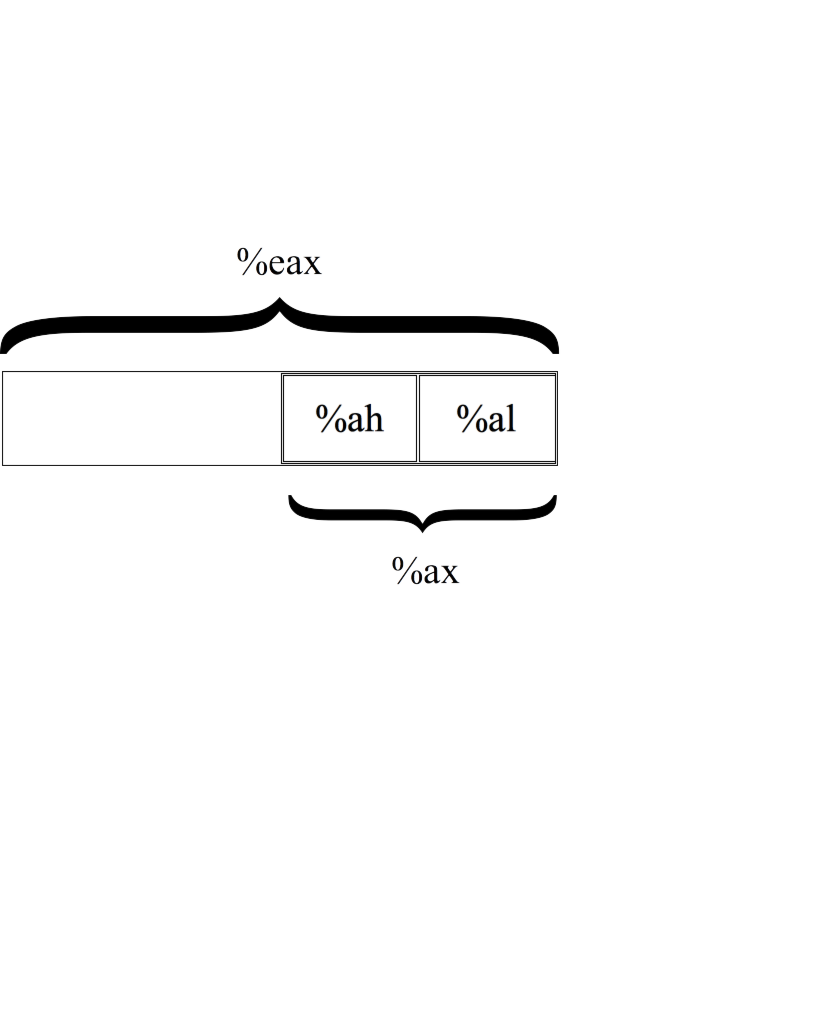
\includegraphics[width=\textwidth]{registerdescription.png}
\end{figure}

For a more comprehensive list of instructions, see \autoref{instructionsappendix}.

\section{Review}

\section{Know the Concepts}

\begin{itemize}\item What does it mean if a line in the program starts with the '\#' character? 
\item What is the difference between an assembly language file and an object code file? 
\item What does the linker do? 
\item How do you check the result status code of the last program you ran? 
\item What is the difference between \icode{movl \$1, {\eaxBare}} and \icode{movl 1, {\eaxBare}}? 
\item Which register holds the system call number? 
\item What are indexes used for? 
\item Why do indexes usually start at 0? 
\item If I issued the command \icode{movl data\_items(,{\ediBare},4), {\eaxBare}} and data\_items was address 3634 and {\ediReg} held the value 13, what address would you be using to move into {\eaxReg}? 
\item List the general-purpose registers. 
\item What is the difference between \icode{movl} and \icode{movb}? 
\item What is flow control? 
\item What does a conditional jump do? 
\item What things do you have to plan for when writing a program? 
\item Go through every instruction and list what addressing mode is being used for each operand. 
\end{itemize}

\section{Use the Concepts}

\begin{itemize}\item Modify the first program to return the value 3. 
\item Modify the \icode{maximum} program to find the minimum instead. 
\item Modify the \icode{maximum} program to use the number 255 to end the list rather than the number 0 
\item Modify the \icode{maximum} program to use an ending address rather than the number 0 to know when to stop. 
\item Modify the \icode{maximum} program to use a length count rather than the number 0 to know when to stop. 
\item What would the instruction \icode{movl \_start, {\eaxBare}} do?  Be specific, based on your knowledge of both addressing modes and the meaning of \icode{\_start}.  How would this differ from the instruction \icode{movl \$\_start, {\eaxBare}}? 
\end{itemize}

\section{Going Further}

\begin{itemize}\item Modify the first program to leave off the \icode{int} instruction line. Assemble, link, and execute the new program.  What error message do you get.  Why do you think this might be? 
\item So far, we have discussed three approaches to finding the end of the list - using a special number, using the ending address, and using the length count.  Which approach do you think is best?  Why?  Which approach would you use if you knew that the list was sorted?  Why? 
\end{itemize} 

